% Options for packages loaded elsewhere
\PassOptionsToPackage{unicode}{hyperref}
\PassOptionsToPackage{hyphens}{url}
%
\documentclass[
  12pt,
]{article}
\usepackage{amsmath,amssymb}
\usepackage{iftex}
\ifPDFTeX
  \usepackage[T1]{fontenc}
  \usepackage[utf8]{inputenc}
  \usepackage{textcomp} % provide euro and other symbols
\else % if luatex or xetex
  \usepackage{unicode-math} % this also loads fontspec
  \defaultfontfeatures{Scale=MatchLowercase}
  \defaultfontfeatures[\rmfamily]{Ligatures=TeX,Scale=1}
\fi
\usepackage{lmodern}
\ifPDFTeX\else
  % xetex/luatex font selection
\fi
% Use upquote if available, for straight quotes in verbatim environments
\IfFileExists{upquote.sty}{\usepackage{upquote}}{}
\IfFileExists{microtype.sty}{% use microtype if available
  \usepackage[]{microtype}
  \UseMicrotypeSet[protrusion]{basicmath} % disable protrusion for tt fonts
}{}
\makeatletter
\@ifundefined{KOMAClassName}{% if non-KOMA class
  \IfFileExists{parskip.sty}{%
    \usepackage{parskip}
  }{% else
    \setlength{\parindent}{0pt}
    \setlength{\parskip}{6pt plus 2pt minus 1pt}}
}{% if KOMA class
  \KOMAoptions{parskip=half}}
\makeatother
\usepackage{xcolor}
\usepackage[margin=1in]{geometry}
\usepackage{graphicx}
\makeatletter
\def\maxwidth{\ifdim\Gin@nat@width>\linewidth\linewidth\else\Gin@nat@width\fi}
\def\maxheight{\ifdim\Gin@nat@height>\textheight\textheight\else\Gin@nat@height\fi}
\makeatother
% Scale images if necessary, so that they will not overflow the page
% margins by default, and it is still possible to overwrite the defaults
% using explicit options in \includegraphics[width, height, ...]{}
\setkeys{Gin}{width=\maxwidth,height=\maxheight,keepaspectratio}
% Set default figure placement to htbp
\makeatletter
\def\fps@figure{htbp}
\makeatother
\setlength{\emergencystretch}{3em} % prevent overfull lines
\providecommand{\tightlist}{%
  \setlength{\itemsep}{0pt}\setlength{\parskip}{0pt}}
\setcounter{secnumdepth}{5}
\usepackage{setspace} \usepackage{amsmath} \usepackage{array} \usepackage{caption} \usepackage{longtable} \usepackage{booktabs} \usepackage{enumitem} \renewcommand{\arraystretch}{1} \captionsetup[table]{skip=5pt} \setstretch{1.5}
\ifLuaTeX
  \usepackage{selnolig}  % disable illegal ligatures
\fi
\usepackage[]{natbib}
\bibliographystyle{apalike}
\IfFileExists{bookmark.sty}{\usepackage{bookmark}}{\usepackage{hyperref}}
\IfFileExists{xurl.sty}{\usepackage{xurl}}{} % add URL line breaks if available
\urlstyle{same}
\hypersetup{
  pdftitle={An Attentional Model of Time Discounting},
  pdfauthor={Zark Zijian Wang},
  hidelinks,
  pdfcreator={LaTeX via pandoc}}

\title{An Attentional Model of Time Discounting}
\author{Zark Zijian Wang}
\date{March 13, 2024}

\begin{document}
\maketitle

\hypertarget{introduction}{%
\section{Introduction}\label{introduction}}

\hypertarget{the-model}{%
\section{The Model}\label{the-model}}

\hypertarget{definition}{%
\subsection{Definition}\label{definition}}

Assume time is discrete. Let
\(s_{0\rightarrow T}\equiv[s_0,s_1,...,s_T]\) denote a reward sequence
that starts delivering rewards at period 0 and ends at period \(T\). At
each period \(t\) of \(s_{0\rightarrow T}\), a specific reward \(s_t\)
is delivered, where \(t\in\{0,1,…,T\}\). Throughout this paper, we only
consider non-negative rewards and finite length of sequence. Therefore,
we set \(s_t \in \mathbb{R_{\geq 0}}\) and \(0\leq T<\infty\). The DM's
choice set is constituted by a range of alternative reward sequences
which start from period 0 and end at some finite period. When making an
intertemporal choice, the DM seeks to find a reward sequence
\(s_{0\rightarrow T}\) in her choice set, which has the highest value
among all alternative reward sequences. To calculate the value of each
reward sequence, we admit the additive discounted utility framework. The
value of \(s_{0\rightarrow T}\) is defined as
\(U(s_{0\rightarrow T})\equiv \sum_{t=0}^T w_{t}u(s_t)\), where \(u(.)\)
is the instantaneous utility function, and \(w_t\) is the decision
weight assigned to \(s_t\). The function \(u(.)\) is twice
differentiable, \(u'>0\) and \(u''<0\).

The determination of \(w_t\) is central to this paper. We believe that
the formation of \(w_t\) is subjective to limited attention.
Specifically, we term a decision weight \(w_t\) as an
\emph{attention-adjusted discount} (AAD) factor if it satisfies
Definition 1.

\textbf{Definition 1}: \emph{Let} \(\mathcal{W}\equiv[w_0,...,w_T]\)
\emph{denote the decision weights for all specific rewards in}
\(s_{0\rightarrow T}\)\emph{.} \(\mathcal{W}\) \emph{is called
attention-adjusted discount factors if for any} \(t\in\{0,1,…,T\}\)

\[\tag{1}
w_t = \frac{d_te^{v(s_t)}}{\sum_{\tau=0}^T d_\tau e^{v(s_\tau)}} 
\]

\emph{where} \(d_t \geq 0\)\emph{,} \(v(.)\) \emph{is a
twice-differentiable function,} \(v'>0\) \emph{and} \(v''<0\)\emph{.}

In intuition, how Definition 1 reflects the role of attention mechanisms
in decision-making can be explained with four points. First, note that
the attention-adjusted discount factors follow a logistic-like
distribution. This is consistent with the prediction of rational
inattention theory. Second, for each \(t\), \(w_t\) is increasing with
\(s_t\), indicating that DM tends to pay more attention to larger
rewards. This is consistent with an empirical phenomenon called
``value-driven attentional capture''. Third, \(w_t\) is ``anchored'' in
the initial weight \(d_t\). We can let \(d_t\) denote the initial weight
that the DM would assign to a reward delivered at period \(t\), without
knowing its realization. This indicates that reallocating attention
based on the newly acquired information is costly. Fourth, note that the
sum of \(w_t\) is fixed at 1, which implies the DM's capacity of
information processing is limited. Being too focused on one reward will
make DM insensitive to another reward in the sequence.

In popular time-discounting models, such as exponential and hyperbolic
discounting, discount factors are typically assumed to be independent of
how each reward is realized in \(s_{0\rightarrow T}\). This type of
discount factors reflects impatience, and can be viewed as initial
weights assigned to each reward when the DM has no information about its
value. That is, we can use them for \(d_t\). By contrast, \(w_t\) in AAD
is influenced by impatience but also reflects the attention allocated to
each specific reward realized in the sequence. Notably, \(w_t\) is
dependent on all rewards realized in \(s_{0\rightarrow T}\). An increase
in \(s_t\) would attract more attention to it, thus the DM would be more
sensitive to \(s_t\), and the attention remained for other rewards in
\(s_{0\rightarrow T}\) will decrease. As a result, she could reduce
other decision weights, i.e.~discount the value of other rewards by a
larger degree.

\hypertarget{related-literature-in-attention}{%
\subsection{Related Literature in
Attention}\label{related-literature-in-attention}}

1 attention bottleneck

2 attentional capture

3 costly information acquisition

\hypertarget{related-literature-in-time-preferences}{%
\subsection{Related Literature in Time
Preferences}\label{related-literature-in-time-preferences}}

\hypertarget{axiomatic-characterizations}{%
\section{Axiomatic
Characterizations}\label{axiomatic-characterizations}}

\hypertarget{the-optimal-discounting-approach}{%
\subsection{The Optimal Discounting
Approach}\label{the-optimal-discounting-approach}}

The first axiomatic characterization of AAD is based on the optimal
discounting model proposed by Noor and Takeoka
\citetext{\citeyear{noor_optimal_2022}; \citeyear{noor_constrained_2023}}.
In one version of their model, they assume that the DM has a limited
capacity of attention (or in their term, ``empathy''), and before
encountering an intertemporal choice problem, the DM naturally focuses
on the current time period. During the choice process, she needs to
split attention over the time interval spanned by an alternative reward
sequence in order to evaluate it. This re-allocation of attention is
cognitive costly. Thus, for each alternative reward sequence, the DM
seeks to maximize the value she can subjectively obtain from the reward
sequence minus the cost incurred by attention re-allocation. In our
setting, we relax the assumption that the DM should initially focuses
all her capacity on the current time; instead, the initial distribution
of decision weights can be flexible.\footnote{There are another two
  difference between us and Noor and Takeoka
  \citetext{\citeyear{noor_optimal_2022}; \citeyear{noor_constrained_2023}}.
  First, in our setting, shifting attention to future periods may also
  reduce the attention to the current period, while this would never
  happen in their settings. Second, for any \(w_t\in[0,1]\), they assume
  that \(f'(w_t)\) could be 0 when \(w_t\) is under a lower bound, could
  be infinity when \(w_t\) is above a upper bound, and is strictly
  increasing in between. To keep simplicity, we assume \(f(.)\) is
  strictly convex, that is, \(f'(w_t)\) is always increasing. Note that
  our assumption is satisfied by many commonly used cost functions (such
  as the power cost function they discussed in their settings, and the
  entropy-based cost function discussed in this paper).} The formal
definition of this optimal discounting problem is given by Definition 2.

Let \(\succsim\) denote the DM's preference for reward sequences. We say
\(\succsim\) has an optimal discounting representation if
\(s_{0\rightarrow T} \succsim s'_{0\rightarrow T'}\) implies
\(\sum_{t=0}^T w_t\cdot s_t \succsim \sum_{t=0}^{T'} w'_t \cdot s'_t\),
and both \(\{w_t\}_{t=0}^T\) and \(\{w'_t\}^{T'}_{t=0}\) are generated
by optimal discounting problems.

\textbf{Definition 2}: \emph{The following optimization problem is
called optimal discounting problem:}

\[
\begin{aligned}
&\max_{\mathcal{W}}\;&&\sum_{t=0}^T w_tv(s_t) - C(\mathcal{W}) \\
&s.t.\; &&\sum_{t=0}^Tw_t \leq M \\
&&& w_t >0 \text{ for all } t\in \{0,1,...,T\}
\end{aligned}
\]

\emph{where} \(C(.)\) \emph{is the cognitive cost function.}
\(C(\mathcal{W})\) \emph{is constituted by time-separable costs, that
is,} \(C(\mathcal{W})=\sum_{t=0}^Tf_t(w_t)\)\emph{, where} \(f_t(.)\)
\emph{is a twice differentiable and strictly convex function.}

We focus on a specification of \(C(.)\), in which we assume that\[
C(\mathcal{W})= \lambda\cdot\sum_{t=0}^T w_t
\ln\left(\frac{w_t}{d_t}\right)
\]

\hypertarget{the-intertemporal-trade-off-approach}{%
\subsection{The Intertemporal Trade-Off
Approach}\label{the-intertemporal-trade-off-approach}}

\hypertarget{implications-in-decision-making}{%
\section{\texorpdfstring{Implications in Decision Making
\label{behavioral}}{Implications in Decision Making }}\label{implications-in-decision-making}}

To illustrate how ADU with Shannon cost function can account for a broad
set of anomalies about time preferences, imagine that a DM receives a
positive detereminstic reward in period \(j\) (and no reward in other
periods). That is, she receives a sequence of rewards
\(X_T=[x_0,x_1,…,x_T]\), where \(x_j>0\) and is certain, and \(x_t = 0\)
for all \(t \neq j\) (both \(j\) and \(t\) are in \(\{0,1,...,T\}\)).

For the convenience of illustration, I assume the DM holds stationary
time preferences before acquiring any information, that is,
\(d_t=\delta^t\). Meanwhile, \(\delta\in(0,1]\), where \(\delta=1\)
implies the initial attention is uniformly distributed across periods.
For simplicity, I define \(v(x_t)=u(x_t)/\lambda\), and set \(v(0)=0\).
Let \(w_t(X_T)\) denote the discounting factor for period \(t\). From
the formula of ADUS we can infer that\[ 
w_j(X_T) = \left\{ \begin{aligned}
& \delta^j \cdot\frac{1}{1+\frac{\delta}{1-\delta}(1-\delta^T)e^{-v(x_j)}}\;, & 0<\delta<1 \\
& \frac{1}{1+T\cdot e^{-v(x_j)}}\; , & \delta=1
\end{aligned}
\right.
\]

Clearly, \(w_j\) is decreasing in \(T\). This offers an account for a
phenomenon called \emph{hidden zero effect}.

\hypertarget{hidden-zero-effect}{%
\subsection{Hidden Zero Effect}\label{hidden-zero-effect}}

The most direct evidence that could support the ADUS model is likely the
hidden zero effect \citep{magen_hidden-zero_2008}. The hidden zero
effect means, supposing people face a small sooner reward (SS) and a
large later reward (LL), they tend to exhibit more patience when SS and
LL are framed as sequences rather than being framed as single-period
rewards. For instance, suppose SS is ``receive £100 today'' and LL is
``receive £120 in 6 months'', and we have

SS\textsubscript{0}: ``receive £100 today and £0 in 6 months''

LL\textsubscript{0}: ``receive £0 today and £120 in 6 months''

people will be more likely to prefer LL\textsubscript{0} over
SS\textsubscript{0} than preferring LL over SS. Subsequent research
(e.g. \citet{read_value_2017}) suggests that the hidden zero effect is
asymmetric. That is, shifting SS to SS\textsubscript{0} and keeping LL
unchanged leads to an increase in patience, whereas shifting LL to
LL\textsubscript{0} and keeping SS unchanged cannot increase patience.
ADUS assumes that, within a sequence, attention is limited and the
weight assigned to each period is anchored in an initial positive
weight. These properties naturally explain the hidden zero effect. To
illustrate, in SS, the DM perceives the length of sequence as ``today''
and allocate no attention to future. Whereas, in SS\textsubscript{0},
she perceives the length as ``6 months''. This makes some attention be
paid to future periods with no reward, and decreases the attention paid
to the only period with positive reward (given attention is limited);
thus, the overall utility of sequence decreases. By contrast, shifting
from LL to LL\textsubscript{0} does not change the length of sequence,
thus does not change overall utility.

The existence of hidden zero effect also provides a hint in selection of
time length \(T\). When evaluating a reward delivered in period \(j\),
the range of \(T\) is \([j,+\infty)\). Any increase in \(T\) will reduce
the overall utility. Thus, when comparing SS and LL, the DM may tend to
set \(T=j\) (the minimum length she can set), in order to maximize the
overall utility. Any period out of this length can be perceived as
irrelevant to the decision; so, she does not need to sample from the
periods after \(j\), when evaluating the given reward. Though,
explicitly mentioning the periods after \(j\) will direct her attention
to those periods, and lead to the hidden zero effect. By setting
\(T=j\), we
have\[ w_T(x_T) = \frac{1}{1+G(T)e^{-v(x_T)}} \]where\[ G(T) = \left\{ \begin{aligned} & \frac{1}{1-\delta}(\delta^{-T}-1) \; ,& 0<\delta<1\\ & T\; ,& \delta=1\ \end{aligned} \right. \]

Given period \(T\) is now the only period with a non-zero reward within
the sequence, I use \(x_T\) to directly represent the whole sequence,
and let \(w_T(x_T)\) denote the discounting factor for period \(T\).
Interestingly, when \(\delta=1\), \(w_T(x_T)\) takes a form similar with
hyperbolic discounting.

\hypertarget{common-difference-effect}{%
\subsection{Common Difference Effect}\label{common-difference-effect}}

A well-known anomaly about time preferences is \emph{common difference
effect}, firstly defined by \citet{loewenstein_anomalies_1992}. Suppose
there are a large later reward \(x_l\) arriving at period \(t_l\)
(denoted by LL) and a small sooner reward \(x_s\) arriving at period
\(t_s\) (denoted by SS), where \(x_l>x_s>0\), \(t_l>t_s>0\). Define
\(V(x,t)=w_t(x_t)v(x_t)\). The common difference effect means,
supposing\(V(x_l,t_l)=V(x_s,t_l)\), we must have
\(V(x_l,t_l+\Delta t)>V(x_s,t_s+\Delta t)\) for any positive integer
\(\Delta t\).

ADUS predicts that, if people are impatient, to observe the common
difference effect, the difference between SS and LL in reward level must
be set significantly larger than the difference in time delay. This is
shown in Proposition 2.

\textbf{Proposition 2}: \emph{In ADUS, if the initial weights are
uniformly distributed, then the common difference effect always holds;
if the initial weights exponentially declines over time, the common
difference effect holds when}
\(v(x_l)-v(x_s)+\ln\frac{v(x_l)}{v(x_s)}>-(t_l-t_s)\ln\delta\)\emph{.}

Proposition 2 is interpreted as follows. When \(\delta = 1\), ADUS
predicts the DM always performs the common difference effect. This is
obvious because discounting factor \(w_T(x_T)\) takes a hyperbolic-like
form. When \(\delta<1\), there are four factors jointly deciding whether
we could observe the common difference effect or not. First, without
considering attentional mechanism, when we extend time delay, each of
\(w_{t_l}(x_l)\) and \(w_{t_s}(x_s)\), i.e.~the discounting factor for
(and attention paid to) the only period with positive reward, declines
in an exponential fashion. Second, without considering newly added time
interval, due to the decline of \(w_{t_l}(x_l)\) and \(w_{t_s}(x_s)\),
the DM frees up some attention and can reallocate it across periods.
Given that in LL, the DM has to wait longer for reward, the periods
where she wait can grab more attention from the released capacity of
attention, compared with those in SS. In other words, an extension of
delay makes she focus more on the waiting time in LL than in SS, which
decreases the preference for LL. Third, the newly added time interval
also grabs some attention from other periods. Note the time delay is
extended by \([t_l,t_l+\Delta t]\) in LL and by \([t_s, t_s+\Delta t]\)
in SS; given \(t_l>t_s\), if people are impatient, the newly added time
interval will receive less attention in LL than in SS, without
considering other factors. This increases the preference for LL. Fourth,
ADU generally assumes that the DM tends to pay more attention to periods
with larger rewards. Given \(x_l>x_s\), the newly added interval grabs
less attention from the period where \(x_l\) is positioned (in LL) than
from the period where \(x_s\) is positioned (in SS). That is, the DM
focuses comparatively more on reward level in LL than in SS, which
mitigates the impact of discounting factor declining. This also
increases the preference for LL. When the impact of the later two
factors succeeds that of the second factor, the DM will perform the
common difference effect.

Notably, if we explicit mention the zeros in LL and SS, extending time
delay always lead to the common difference effect.

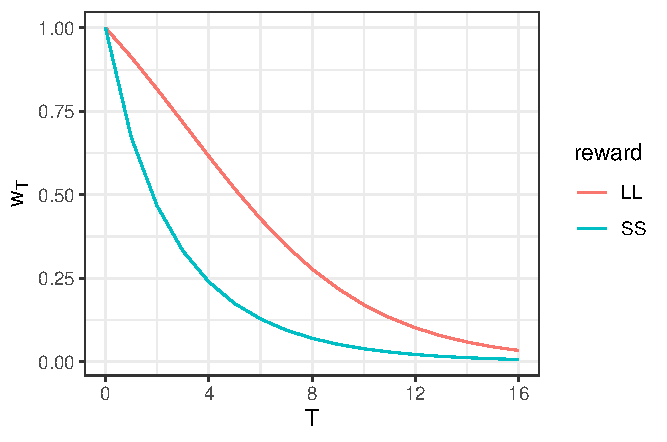
\includegraphics{images/weight_LLvSS.pdf}

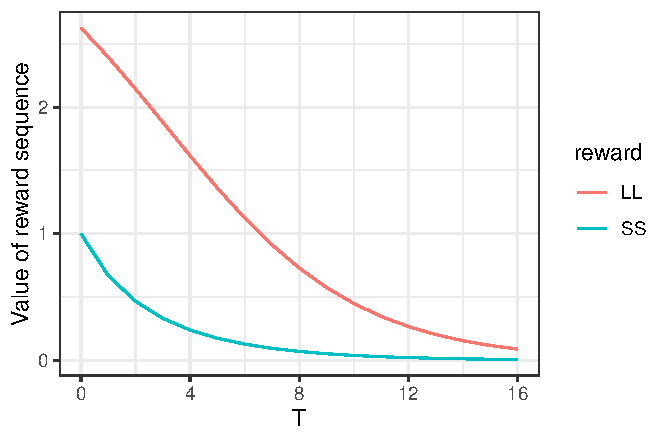
\includegraphics{images/value_LLvSS.pdf}

\hypertarget{magnitude-effect}{%
\subsection{Magnitude Effect}\label{magnitude-effect}}

The \emph{magnitude effect} is another well-known anormaly about time
preferences. Assuming we have \(t_l\), \(t_s\), \(x_s\) fixed, and want
to find a \(x_l\) such that \(V(x_l,t_l) \equiv V(x_s,t_s)\), the
magnitude effect implies that, if we increase \(x_s\), then the
\(x_l/x_s\) that makes the equality valid will decrease.

In standard discounted utility model, the magnitude effect requires the
elasticity of utility function to increase with the reward level
\citep{loewenstein_anomalies_1992}. This requirement might be too
restrictive, so that many commonly used utility functions (such as power
or CARA utility function) does not satisfy it. By contrast, in ADU
model, DM is generally assumed to attend more to periods with larger
rewards. This implies that when comparing SS and LL, she exhibits more
patience towards larger reward level, which is naturally compatible with
the magnitude effect \citep{noor_intertemporal_2011, noor_optimal_2022}.
By Proposition 3, I focus on ADU with Shannon cost function, and show
how this requirement for curvature of utility function can be relaxed in
this setting.

\textbf{Proposition 3}: \emph{Define} \(v(x)\equiv u(x)/\lambda\)
\emph{as the utility function. In ADUS, the magnitude effect always
holds true when function} \(v(x)\) \emph{satisfies}\[
RRA_v(x)\leq 1-\frac{e_v(x)}{v(x)+1}
\]\emph{where} \(RRA_v(x)\) \emph{is the relative risk aversion
coefficient of} \(v(x)\)\emph{,} \(e_v(x)\) \emph{is the elasticity of}
\(v(x)\) \emph{to} \(x\)\emph{.}

Note that Proposition 3 is a very broad condition. In Corollary 1 and
Corollary 2, I show that power utility function and CARA utility
function both satisfy this condition in most cases.

\textbf{Corollary 1}: Suppose \(v(x)=x^\gamma/\lambda\), where
\(0<\gamma<1\) and \(\lambda>0\). Then magnitude effect holds true for
any \(x\in \mathbb{R}_{>0}\).

\textbf{Corollary 2}: Suppose \(v(x)=(1-e^{-\gamma x})/\lambda\), where
\(\gamma>0\) and \(\lambda>0\). The magnitude effect holds true for any
\(x\geq \frac{1+\eta}{\gamma}\), where \(\eta>0\) and
\(\eta e^{1+\eta}-\eta=1\) (it can be calculated that
\(\eta \approx 0.35\)).

\hypertarget{concavity-of-time-discounting}{%
\subsection{Concavity of Time
Discounting}\label{concavity-of-time-discounting}}

Many time discounting models assumes discount function is convex in time
delay, e.g.~exponential and hyperbolic discounting. This style of
discount function predicts DM is \emph{risk seeking over time
lotteries}. That is, suppose a deterministic reward of level \(x\) is
delivered in period \(t_l\) with probability \(\pi\) and delivered in
period \(t_s\) with probability \(1-\pi\) (\(0<\pi<1\), \(c>0\)); while
another deterministic reward, of the same level, is delivered in a
certain period \(t_m\), where \(t_m=\pi t_l +(1-\pi) t_s\). The DM
should prefer the former reward to the latter reward. However, some
experimental studies, such as \citet{onay_intertemporal_2007} and
\citet{dejarnette_time_2020}, suggest that people are often \emph{risk
averse over time lotteries}, i.e.~preferring the reward delivered in a
certain period.

One way to accommodate the evidence about risk aversion over time
lotteries, as is suggested by \citet{dejarnette_time_2020}, is to modify
the convexity (concavity) of discount function. Under a general EDU
framework, DM is risk averse over time lotteries when
\(\pi w_{t_l}(x)+(1-\pi)w_{t_s}(x)<w_{t_m}(x)\). Fixing \(t_s\) and
\(t_l\), the inequality suggests \(w_{t_m}(c)\) is concave in \(t_m\).
In reverse, being risk seeking over time lotteries suggests
\(w_{t_m}(x)\) is convex in \(t_m\). Notably,
\citet{onay_intertemporal_2007} find that people are more likely to be
risk averse over time lotteries when \(\pi\) is small, and to be risk
seeking over time lotteries when \(\pi\) is large. Given that when
\(\pi\) gets larger, \(t_m\) is also larger, we can conclude that the
discount function may be concave in delay for the near future but convex
for the far future. Moreover, \citet{takeuchi_non-parametric_2011} also
find evidence that support this shape of discount function.

In Proposition 4, I show that ADUS can produce such a shape of discount
function as long as the reward level \(x\) is large enough.

\textbf{Proposition 4}: In ADUS, \emph{if} \(\delta =1\)\emph{, then the
discount function is convex in} \(t\)\emph{. If} \(0<\delta<1\)\emph{,
then there are a reward threshold} \(\underline{x}\) \emph{and a time
threshold} \(\underline{t}\) \emph{such that}

\begin{enumerate}
\def\labelenumi{\arabic{enumi})}
\tightlist
\item
  \emph{when} \(x\leq \underline{x}\)\emph{, the discount function is
  convex in} \(t\)\emph{;}
\item
  \emph{when} \(x > \underline{x}\)\emph{, the discount function is
  convex in} \(t\) \emph{given} \(t\geq \underline{t}\)\emph{, and it is
  concave in} \(t\) \emph{given} \(t<\underline{t}\)\emph{.}
\end{enumerate}

\emph{It can be derived that}
\(v(\underline{x})=\ln(\frac{2}{1-\delta})\)\emph{, and}
\(\underline{t}=\frac{\ln[(1-\delta)e^{v(x)}-1]}{-\ln\delta}\)\emph{.}

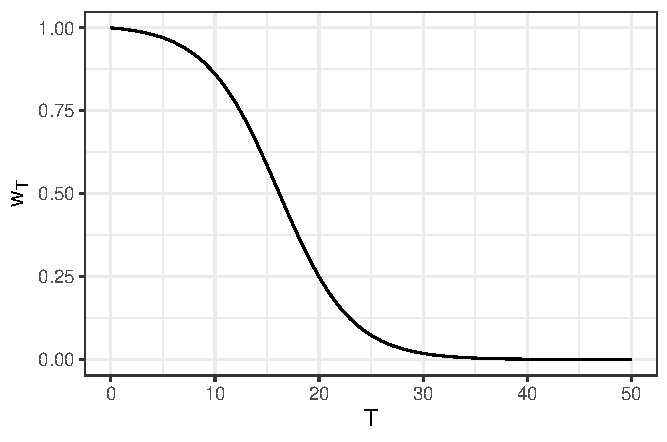
\includegraphics{images/concavity_discount.pdf}

\hypertarget{s-shaped-value-function}{%
\subsection{S-Shaped Value Function}\label{s-shaped-value-function}}

In prospect theory, \citet{kahneman_prospect_1979} propose an S-shaped
value function that is convex for losses and concave for gains. Since
that, S-shaped value functions have been widely embraced by behavioral
economists. More recent theories have provided further justifications
for it, including reference-dependent utility in a broad sense
\citep{koszegi_model_2006}, and efficient coding of values
\citep{frydman_efficient_2021}. Here, I provide an account based on
selective attention to time periods.

Suppose a DM is faced with a choice between a risky lottery and a fixed
amount of money. When making this choice, she does not obtain any money
from either option. Thus, she perceives the outcome of each option as
something that will happen in the future. She allocate her attention
between the present period and the period when she may receive the
money. Assume that she perceives the outcome will be realized in period
\(t\), and in a certain state, the option she chooses yields reward
\(x\), then we can use the attentional discounted utility \(V(x,t)\) to
represent the value function. I derive the conditions in which ADUS can
produce a S-shaped value function in Proposition 5.

\textbf{Proposition 5}: \emph{Suppose} \(t\geq1\)\emph{,}
\(\frac{d}{dx}\left(\frac{1}{v'(x)}\right)\) \emph{is continuous in}
\((0,+\infty)\)\emph{, in ADUS,}

\begin{enumerate}
\def\labelenumi{\arabic{enumi})}
\item
  \emph{there exists a threshold} \(\bar{x}\) \emph{in} \((0,+\infty)\)
  \emph{such that} \(V(x,t)\) \emph{is strictly concave in} \(x\)
  \emph{when} \(x\in [\bar{x},+\infty)\)\emph{;}
\item
  \emph{if} \(\frac{d}{dx}\left(\frac{1}{v'(x)}\right)\) \emph{is
  right-continuous at} \(x=0\)\emph{, and}
  \(\frac{d}{dx}\left(\frac{1}{v'(0)}\right)<1\)\emph{, then there
  exists a threshold} \(x^*\) \emph{in} \((0, \bar{x})\) \emph{such
  that, for any} \(x\in (0,x^*)\)\emph{,} \(V(x,t)\) \emph{is strictly
  convex in} \(x\)\emph{;}
\item
  \emph{there exist a hyper-parameter} \(\lambda^*\) \emph{and an
  interval} \((x_1,x_2)\) \emph{such that, if}
  \(\lambda<\lambda^*\)\emph{, for any} \(x\in(x_1,x_2)\)\emph{,}
  \(V(x,t)\) \emph{is strictly convex in} \(x\)\emph{, where}
  \(\lambda^*>0\) \emph{and} \((x_1,x_2)\subset(0,\bar{x})\)\emph{.}
\end{enumerate}

Proposition 5 implies, if the derivative of \(\frac{1}{v'(x)}\)
converges to a small number when \(x\rightarrow 0^+\), or the unit cost
of information \(\lambda\) is small enough, value function \(V(x,t)\)
will perform an S shape in some interval of \(x\). At the intuition
level, note that \(V(x,t)=w_t(x)v(x)\). When the level of reward \(x\)
grows, both the instantaneous utility of it, i.e.~\(v(x)\), and the
discounting factor assigned to it, i.e.~\(w_t(x)\), can increase. These
functions are both concave in \(x\): when the level of reward is small,
they both grow fast. So, it is possible that their product is convex in
this case. By contrast, when the level of reward is large, they grow
slowly, so their product keeps concave.

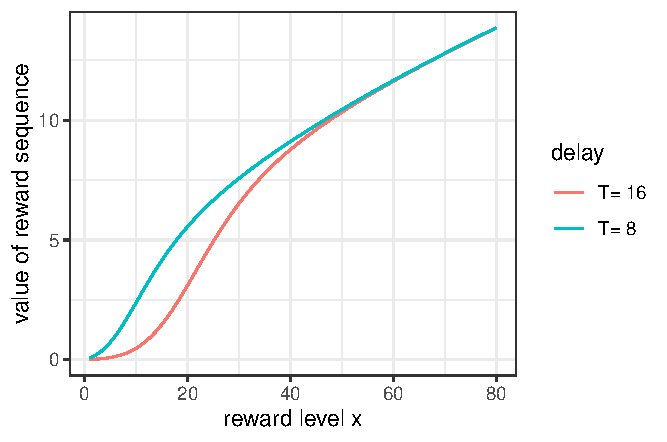
\includegraphics{images/S_shaped_value.pdf}

\hypertarget{inseparability-of-sequences}{%
\subsection{Inseparability of
Sequences}\label{inseparability-of-sequences}}

Let \(x\) and \(y\) denote two 2-period risky reward sequences. For
\(x\), the realized sequence is {[}£100,£100{]} with probability 1/2,
and is {[}£3,£3{]} with probability 1/2. For \(y\), the realized
sequence is {[}£3,£100{]} with probability 1/2, and is {[}£100,£3{]}
with probability 1/2. Classical models of intertemporal choice typically
assume the separability of potentially realized sequences. This implies
that the DM is indifferent between \(x\) and \(y\). However,
\citet{andersen_multiattribute_2018} find evidence of
\emph{intertemporal correlation aversion}, that is, people often prefer
\(y\) to \(x\).

ADU can naturally yield intertemporal correlation aversion. For
simplicity, suppose the initial attention is uniformly distributed
across the two periods. For \(x\), under each potentially realized
sequence, the DM equally weights each period. For \(y\), DM tends to
assign more weight to the period with a reward of £100 (suppose that
weight is \(w\)). Then the value of \(x\) is
\(\frac{1}{2} u(100) + \frac{1}{2} u(3)\) and the value of \(y\) is
\(w\cdot u(100) +(1-w) \cdot u(3)\). Given that \(x>\frac{1}{2}\), the
DMs should strictly prefer \(y\) to \(x\).

\begin{itemize}
\tightlist
\item
  Other evidence related to inseparability: common sequence effect,
  (reverse) mere token effect, magnitude-increasing temporal sensitivity
\end{itemize}

\hypertarget{the-role-of-attention-in-inconsistent-planning}{%
\section{The Role of Attention in Inconsistent
Planning}\label{the-role-of-attention-in-inconsistent-planning}}

\hypertarget{attention-grabbing-and-updating}{%
\subsection{Attention Grabbing and
Updating}\label{attention-grabbing-and-updating}}

Suppose a DM has budget \(m\) (\(m>0\)) and is considering how to spend
it over different time periods. We can use a reward sequence \(x\) to
represent this decision problem, where the DM's spending in period \(t\)
is \(x_t\). In period 0, she wants to find a \(x\) such
that\[ \tag{3} \max_{x}\;\sum_{t=0}^T w_t u(x_t)\quad s.t. \;\sum_{t=0}^T x_t = m   \]

where \(w_t\) is the attention-adjusted discounting factor in period
\(t\). I assume
\(w_t=\delta^t e^{u(x_t)/\lambda}/\sum_{t=\tau}^T \delta^{\tau} e^{u(x_\tau)/\lambda}\)
and there is no risk under this setting.

In models like exponential and hyperbolic discounting, the discounting
factor of a future period is consistently smaller than that of the
current period. Thus, the DM should spend more at the present than in
the future. By contrast, in ADU, when increasing the spending in a
certain period, the discounting factor corresponding to that period
should also increase. So it is possible that the DM spends more in the
future and that a future period has a greater discounting factor than
the current period. This is consistent with
\citet{loewenstein_preferences_1993} that find people sometimes prefer
improving sequences to declining sequences.

ADU suggests there are two mechanisms that can help explain why people
may perform dynamically inconsistent behavior. The first is
\emph{attention-grabbing effect}, that is, keeping the others equal,
when we increase \(x_t\) (which lead to an increase in \(w_t\)), the
discounting factor in any other period should decrease due to limited
attention. After omitting a previous period from the decision problem in
Equation (3), the DM can assign more weights to remaining periods; thus,
the attention-grabbing effect is enhanced. The increased
attention-grabbing effect will offset some benefit of increasing
spending toward a certain period. Therefore, when the DM prefers
improving sequences, the attention-grabbing effect will make her perform
a present bias-like behavior (always feeling that she should spend more
at the present than the original plan); when the DM prefers declining
sequences, this effect will maker her perform a future bias-like
behavior (always feeling she should spend more in the future).

The second mechanism is \emph{initial attention updating}. As is assumed
above, in period 0, prior to evaluating each reward sequence, the DM's
initial weight on period \(t\) is proportional to \(\delta^t\); after
evaluation, the weight becomes being proportional to
\(\delta^t e^{u(x_t)/\lambda}\). In period 1, if she implements the
evaluation based on the information attained in period 0, the initial
weight should be updated to being proportional
\(\delta^t e^{u(x_t)/\lambda}\); thus, the weight after evaluation
should become being proportional to \(\delta e^{2u(x_t)/\lambda}\). As a
result, the benefit of increasing spending toward a certain period gets
strengthened. The updated initial attention can make those who prefer
improving sequences perform present bias and those who prefer declining
sequences perform future bias.

Both the attention-grabbing effect and initial attention updating are
affected by the curvature of utility function. They jointly decide which
behavior pattern that people should perform in dynamics.

\textbf{Proposition 6} (\emph{spread-consistency correlation}) Suppose
\(\succsim\) has a ADU representation and satisfies Axiom 2-4. If there
exist \(b\) and \(S_T\) such that, for any \(b'\) and \(S_T'\),
\(bS_T\succsim b'S_T'\), where
\(b+\sum_{t=0}^Ts_t=b'+\sum_{t=0}^Ts_t'\), then for any \(S'_T\), we
have \[S_T \succsim S_T' \Longleftrightarrow b\sim S_T\]where
\(\sum_{t=0}^Ts_t=\sum_{t=0}^Ts_t'\).

Proposition 6 implies that, when allocating a consumption budget across
time periods, the DM keeps her choice dynamically consistent if and only
if she performs a strong preference for spread. Given that people are
typically assumed to be impatient (preferring a declining sequence), one
intuitive interpretation of Lemma 2 is that the less impatient a DM is
in the present, the less inclined she is to deviate from the original
choice in the future.

\hypertarget{discussion}{%
\section{Discussion}\label{discussion}}

\hypertarget{conclusion}{%
\section{Conclusion}\label{conclusion}}

\renewcommand\refname{Reference}
  \bibliography{reference.bib}

\end{document}
